\documentclass[11pt]{article}

% ================================================================ packages
\usepackage{lmodern}
\usepackage[T1]{fontenc}
\usepackage[utf8]{inputenc}
\usepackage[margin=1in]{geometry}
\usepackage{amsmath,amssymb}
\usepackage{booktabs,longtable,array}
\usepackage{graphicx}
\usepackage{xcolor}
\usepackage{microtype}
\usepackage{enumitem}
\usepackage[most]{tcolorbox}
\usepackage{titlesec}
\usepackage{listings}
\usepackage{fancyhdr}
\usepackage{tikz}
\usetikzlibrary{arrows.meta,positioning,calc}
\usepackage[colorlinks=true,linkcolor=accent,urlcolor=accent,citecolor=accent]{hyperref}

\urlstyle{tt}
\def\UrlBreaks{\do\/\do\-\do\_\do\.}
\newcommand{\cmd}[1]{\nolinkurl{#1}}

% ================================================================ palette
\definecolor{accent}{HTML}{0B5394}
\definecolor{accentdark}{HTML}{073763}
\definecolor{rulegray}{HTML}{B7B7B7}
\definecolor{codebg}{HTML}{F5F6F8}
\definecolor{codeframe}{HTML}{D9DCE1}
\definecolor{notebg}{HTML}{EAF2FB}
\definecolor{warnbg}{HTML}{FBE9E7}
\definecolor{warnframe}{HTML}{C0392B}
\definecolor{okgreen}{HTML}{1E8449}
\definecolor{wiporange}{HTML}{B9770E}

% ================================================================ section styling
\titleformat{\section}{\Large\bfseries\color{accentdark}}{\thesection}{0.6em}{}
\titleformat{\subsection}{\large\bfseries\color{accent}}{\thesubsection}{0.6em}{}
\titleformat{\subsubsection}{\normalsize\bfseries\color{accentdark}}{\thesubsubsection}{0.6em}{}
\titlespacing*{\section}{0pt}{2.2ex plus 1ex minus .2ex}{1.2ex plus .2ex}

% ================================================================ headers
\pagestyle{fancy}\fancyhf{}
\lhead{\small\color{accentdark}Differentiable Engine MDO --- Plan \& Tracker}
\rhead{\small\thepage}
\renewcommand{\headrulewidth}{0.4pt}

% ================================================================ listings
\lstset{basicstyle=\ttfamily\footnotesize,breaklines=true,frame=single,
  backgroundcolor=\color{codebg},rulecolor=\color{codeframe},
  showstringspaces=false,columns=fullflexible,keepspaces=true}

% ================================================================ callouts
\newtcolorbox{keybox}{colback=notebg,colframe=accent,boxrule=0.8pt,
  arc=2pt,left=6pt,right=6pt,top=5pt,bottom=5pt}
\newtcolorbox{warnbox}{colback=warnbg,colframe=warnframe,boxrule=0.8pt,
  arc=2pt,left=6pt,right=6pt,top=5pt,bottom=5pt}

% ================================================================ status badges (build-safe, no extra pkgs)
\newcommand{\badge}[2]{{\color{#1}\rule[-0.05ex]{1.0ex}{1.0ex}}\,\small #2}
\newcommand{\stDone}{\badge{okgreen}{done}}
\newcommand{\stWip}{\badge{wiporange}{wip}}
\newcommand{\stTodo}{\badge{rulegray}{to do}}

% ================================================================ math shorthands
\newcommand{\dd}[2]{\frac{\mathrm{d}#1}{\mathrm{d}#2}}
\newcommand{\pd}[2]{\frac{\partial #1}{\partial #2}}
\newcommand{\Rt}{R_t}
\newcommand{\mdot}{\dot m}
\newcommand{\cstar}{c^{*}}
\newcommand{\vc}[1]{\mathbf{#1}}

\title{\vspace{-1.2cm}\textbf{\color{accentdark}Differentiable Multidisciplinary Design Optimization\\[2pt]
of an Electric-Pump-Fed Liquid Rocket Engine}\\[6pt]
\large Formulation, Literature Basis, and Implementation Tracker for LREKit}
\author{Ibrahim Shahid}
\date{\today\quad\textbullet\quad Version 0.1 (living document)}

\begin{document}
\maketitle
\thispagestyle{fancy}

\begin{keybox}
\textbf{Purpose.} A single reference for the differentiable engine-MDO workstream:
the mathematical formulation, the governing physics of each discipline, the
literature each modelling choice rests on, and a phase/gate table to track
build progress. It supersedes the loose plan notes and folds in the
literature verification of July 2026.\\[3pt]
\textbf{Build.} \cmd{latexmk -pdf Differentiable_Engine_MDO_Plan.tex}
(or \cmd{pdflatex} twice for the table of contents).\\[3pt]
\textbf{Status legend.} \stDone{} complete \quad \stWip{} in progress \quad \stTodo{} not started.
\end{keybox}

\tableofcontents
\vspace{4pt}\hrule

% =====================================================================
\section{Scope and one-paragraph statement}

We build a \emph{multidisciplinary-feasible} (MDF), end-to-end differentiable
model of the continuous states of an electric-pump-fed liquid rocket engine,
and drive it with a gradient-based constrained optimizer. Discrete hardware
choices (channel/blade/stage counts, materials, architecture) are handled by an
\emph{outer enumeration}, not by relaxing integers. ``End-to-end differentiable''
means \emph{exact total derivatives of the discretized engineering models};
it does \emph{not} mean differentiating CAD Boolean operations, integer counts,
or arbitrary software branches. The engineering novelty is the coupled
\emph{total} derivative through the converged engine state; the physical novelty
is the interaction of engine-level optima with the Rao nozzle
\emph{existence boundary} under perfect- and real-gas thermochemistry.

% =====================================================================
\section{Corrected literature foundation}
\label{sec:lit}

The plan's architecture is justified paper-by-paper. The mappings below were
checked against the source PDFs in \cmd{propulsion_texts/} (text extracted and
read, not inferred from filenames). One load-bearing attribution was corrected.

\subsection{The Rao 1958 vs.\ Rao 1999 correction (load-bearing)}

\begin{warnbox}
\textbf{Correction.} The claim ``the contour must remain an implicit solved
state, not a B\'ezier lookup'' is \emph{physically correct} but was attributed
to the wrong source. \textbf{Rao 1958}~\cite{rao1958} establishes that the
optimum contour is a constrained variational solution --- the control surface is
forced to be a characteristic surface and thrust is maximized at fixed mass flow
via Lagrange multipliers $\lambda_2,\lambda_3$, with Rao stating the optimality
condition ``is \emph{implicit} in the solution'' of the governing equations.
But Rao 1958 does \emph{not} require an engine MDO to re-solve the contour
implicitly at every iterate; the Rao/TOP parabola is a \emph{validated
approximation} to that same optimum. The requirement for the implicit contour
comes from \textbf{Rao 1999}~\cite{rao1999}, which defines the \emph{boundary of
the valid (shock-free) region} --- the ``invalid region'' where the
optimum-thrust control surface can no longer be computed normally. \emph{That
boundary is the ``Rao cliff''}; a B\'ezier lookup has no such boundary. Two
consequences: (i) cite Rao 1999, not Rao 1958, for the implicit-contour
requirement; (ii) Rao 1999 already computes how \emph{equilibrium chemistry
shifts the valid-region boundary}, so it is direct prior art for
RQ4 (real-gas migration).
\end{warnbox}

\noindent\textbf{Design consequence --- two contour fidelities, switched by the question.}
\begin{itemize}[leftmargin=1.4em,itemsep=2pt]
\item \emph{Bulk MDO sweeps} (mass--$I_{sp}$ Pareto front): use the analytic
Rao/TOP B\'ezier contour. It is smooth, cheap, endpoint-exact, and adequate
for the value-of-coupling questions.
\item \emph{Existence-boundary and exact-vs-TOP studies}: use the implicit
variational/MOC boundary-value contour as a solved state. Total derivatives to
the \emph{manufacturable wall} here still require the differentiable
kernel/BDE march (the ``J3b'' item); until that lands, the kernel $BD$ is a
frozen artifact and wall-coordinate sensitivities are unavailable. Keep this on
the critical path only for the runs that need it.
\end{itemize}

\subsection{Verified source identities}

\begin{center}
\small
\begin{tabular}{@{}p{2.7cm}p{3.3cm}p{6.9cm}@{}}
\toprule
\textbf{Cited as} & \textbf{File} & \textbf{Verified identity} \\
\midrule
NASA SP-8087 & \cmd{19730022965.pdf} & ``Liquid Rocket Engine Fluid-Cooled Combustion Chambers'' --- confirmed (text layer). \\
NASA SP-8109 & \cmd{fuel\_pump\_design/19740020848.pdf} & ``\dots Centrifugal Flow Turbopumps'' --- confirmed. \\
NASA SP-8052 & \cmd{fuel\_pump\_design/19710025474.pdf} & ``\dots Turbopump Inducers'' --- confirmed. \\
NASA SP-8089 & \cmd{pintle\_injector/19760023196.pdf} & \emph{Image scan, no text layer} --- identity not text-verifiable; consistent with ``\dots Injectors''. Requires OCR to parse. \\
Rao 1958 & \cmd{rao1958.pdf} & ``Exhaust Nozzle Contour for Optimum Thrust''. Page~1 is a spillover references page from the preceding journal article; Rao's text begins p.~2. \\
Rao 1999 & \cmd{rao1999.pdf} & ``Nozzle Optimization for Space-Based Vehicles'' --- valid/invalid region, equilibrium-chemistry boundary. \\
\bottomrule
\end{tabular}
\end{center}

\subsection{Verified discipline mappings}

\begin{center}
\small
\begin{tabular}{@{}p{3.0cm}p{5.2cm}p{4.6cm}@{}}
\toprule
\textbf{Source} & \textbf{Claim used in plan} & \textbf{Verification} \\
\midrule
Pizzarelli 2011~\cite{pizzarelli2011} & Channel aspect ratio governs stratification, rib conduction, wall temperature, $\Delta p$; throat-only thermal is insufficient. & Confirmed: quasi-2-D (1-D coolant mass/momentum $+$ 2-D energy), $k=h/b$ up to $8$ at throat; higher $k$ lowers hot-gas wall temperature via ribs. \\
Son 2017~\cite{son2017} & Real minimum-area transition (tip-opening vs.\ center-gap limited); model as two branches, not \cmd{min()}. & Confirmed: center-gap area vs.\ minimum orifice near pintle tip; explicit ``transition of the minimum area''. \\
Lee 2021~\cite{lee2021} & Battery mass has separate power- and energy-limited terms; burn duration is an optimization variable. & Confirmed: power density and energy/discharge-time both drive battery mass; voltage droop at short discharge. \\
SP-8087~\cite{sp8087} & Regen cooling as coupled allocation of coolant, $\Delta p$, wall temperature, geometry, life. & Confirmed. \\
SP-8109/8052~\cite{sp8109,sp8052} & Pump RPM and inducer suction/mechanics as a simultaneous constrained design. & Confirmed. \\
\bottomrule
\end{tabular}
\end{center}

% =====================================================================
\section{System boundary and mass ledger}

The optimized system runs from the tank outlets and electrical source to the
nozzle exit. Everything excluded must appear explicitly (as zero or as a fixed
allowance) in the ledger, so tanks and trajectory can be added later without
changing the engine formulation.

\begin{center}
\small
\begin{tabular}{@{}p{6.4cm}p{6.4cm}@{}}
\toprule
\textbf{Inside boundary} & \textbf{Initially excluded (ledger placeholders)} \\
\midrule
Fuel/oxidizer pumps, inducers, motors, inverters, battery & Propellant tanks, pressurant \\
Feed-line and manifold pressure losses & Vehicle structure, TVC \\
Regenerative cooling circuit & Valves, ignition, avionics \\
Pintle injector, chamber, converging section & Transient combustion CFD \\
Rao nozzle and delivered performance & Blade-resolved pump CFD, CAD Booleans \\
\bottomrule
\end{tabular}
\end{center}

\noindent Reported masses: thrust-chamber/nozzle hardware, injector, pumps$+$inducers,
motors$+$inverters, battery, total installed propulsion-package mass, and mission
propellant consumed.

% =====================================================================
\section{Mathematical formulation}
\label{sec:math}

\subsection{Variables and states}
Let $a$ be discrete architecture choices, $x_h$ shared continuous hardware
variables, $x_k$ controls at operating point $k$, and $y_k$ the coupled physical
states at point $k$:
\begin{equation}
x_h=\big[P_c,\,O/F,\,\varepsilon,\,L_\%,\,R_d/\Rt,\,L^{*},\,A_c/A_t,\,
t_\mathrm{hot},w_c,h_c,\beta_\mathrm{regen},\,\tfrac{\Delta p_f}{P_c},\tfrac{\Delta p_o}{P_c},\,
D_\mathrm{pintle},N_f,N_o\big],
\end{equation}
where $N_f,N_o$ are continuous pump speeds (not blade counts). The minimum
implicit state is
\begin{equation}
y=\big[\,u_\mathrm{Rao},\,\Rt,\,\eta_{\cstar},\,T_{c,i},P_{c,i},q_i,T_{wg,i},T_{wc,i},\,
Q_f,H_f,Q_o,H_o\,\big].
\end{equation}
Relations that are naturally explicit stay explicit; we do not enlarge the
nonlinear system merely to appear ``coupled.''

\subsection{The MDF optimization problem}
\begin{equation}
\begin{aligned}
\min_{a,\,x_h,\,\{x_k\}}\quad & J\big(x_h,\{x_k\},\{y_k\}\big)\\
\text{s.t.}\quad
& R_k(y_k,x_h,x_k;a)=0 && \text{(engine state, each point $k$)}\\
& g_k(y_k,x_h,x_k;a)\le 0 && \text{(local constraints)}\\
& G_\mathrm{mission}(\{y_k\},x_h)\le 0. && \text{(shared/mission constraints)}
\end{aligned}
\label{eq:mdf}
\end{equation}
MDF: every optimizer evaluation receives a \emph{converged} engine state
$y_k(x)$ satisfying $R_k=0$. This is the standard multidisciplinary-feasible
architecture~\cite{martinsLambe2013,martinsNing2021}.

\subsection{Total derivatives by implicit differentiation}
We never differentiate through solver iterations. At a converged state
$R(y,x)=0$ the implicit function theorem gives
\begin{equation}
R_y\,\dd{y}{x}+R_x=0
\quad\Longrightarrow\quad
\dd{y}{x}=-R_y^{-1}R_x,
\label{eq:ift}
\end{equation}
so for any output $f(y,x)$,
\begin{equation}
\dd{f}{x}=f_x-f_y\,R_y^{-1}R_x .
\label{eq:total}
\end{equation}
The bracketed inverse is realized in one of two modes. \textbf{Direct/forward}
solves $R_y\,\phi=-R_x$ for the state sensitivities $\phi=\mathrm{d}y/\mathrm{d}x$
(cost $\propto n_x$ linear solves). \textbf{Adjoint/reverse} solves
\begin{equation}
R_y^{\!\top}\lambda=f_y^{\!\top},
\qquad
\dd{f}{x}=f_x-\lambda^{\!\top}R_x,
\label{eq:adjoint}
\end{equation}
at cost $\propto n_f$ solves (one per objective/aggregated constraint). This is
the unified-derivatives view of Martins \& Hwang and the MAUD architecture in
OpenMDAO~\cite{martinsHwang2013,hwangMartins2018,gray2019}.

\begin{keybox}
\textbf{Mode selection (honest sizing).} The first engine has
$n_x\!\approx\!12$--$20$ continuous variables but \emph{hundreds} of stationwise
constraints. This is \textbf{not} high-dimensional MDO: adjoint has no
asymptotic edge here. Use \emph{forward/direct} total derivatives to assemble
the full constraint Jacobian in one pass; use the \emph{adjoint} only for scalar
objectives. The real win over finite differences is exactness and freedom from
step-size noise, plus tight KKT satisfaction --- not conquering dimensionality.
\end{keybox}

\subsection{Differentiating converged fixed points}
Feedback closures (the $\eta_{\cstar}$ loop, the pump operating point) are
fixed points $y=T(y,x)$ or roots $F(y,x)=0$. Differentiate the \emph{converged}
root via \eqref{eq:ift}, implemented with a \cmd{custom\_root}/
\cmd{custom\_fixed\_point} construct~\cite{blondel2022,optimistix2024}, never by
unrolling the iteration. Inner residuals must be converged at least
$100\times$ tighter than the optimizer feasibility tolerance, or the
``exact'' gradient is exact for the wrong equation.

% =====================================================================
\section{Coupling structure}
\label{sec:coupling}

\begin{figure}[h]
\centering
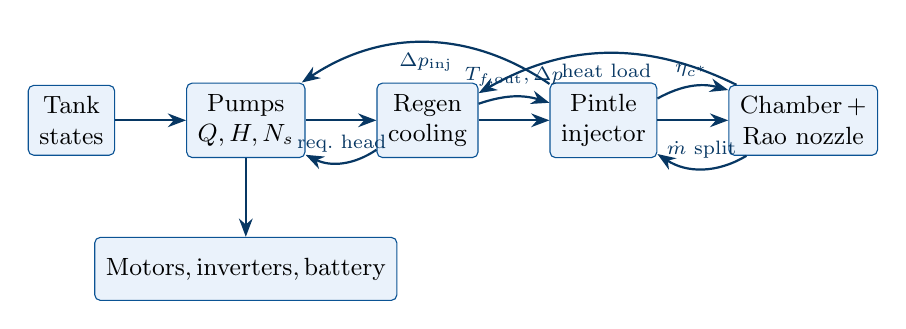
\begin{tikzpicture}[
  >={Stealth[length=2mm]},
  box/.style={draw=accent,fill=notebg,rounded corners=2pt,inner sep=4pt,
              font=\small,minimum height=8mm,align=center},
  fb/.style={accentdark,thick},
  node distance=6mm and 9mm]
\node[box] (T) {Tank\\states};
\node[box,right=of T] (P) {Pumps\\$Q,H,N_s$};
\node[box,right=of P] (C) {Regen\\cooling};
\node[box,right=of C] (I) {Pintle\\injector};
\node[box,right=of I] (N) {Chamber\,+\\Rao nozzle};
\node[box,below=10mm of P] (E) {Motors,\,inverters,\,battery};
\draw[fb,-{Stealth}] (T)--(P); \draw[fb,-{Stealth}] (P)--(C);
\draw[fb,-{Stealth}] (C)--(I); \draw[fb,-{Stealth}] (I)--(N);
\draw[fb,-{Stealth}] (P)--(E);
% feedback arcs
\draw[fb,-{Stealth}] (N) to[bend right=28] node[below,font=\scriptsize]{heat load} (C);
\draw[fb,-{Stealth}] (N) to[bend left=32] node[above,font=\scriptsize]{$\mdot$ split} (I);
\draw[fb,-{Stealth}] (I) to[bend left=22] node[above,font=\scriptsize]{$\eta_{\cstar}$} (N);
\draw[fb,-{Stealth}] (C) to[bend left=18] node[above,font=\scriptsize]{$T_{f,\mathrm{out}},\Delta p$} (I);
\draw[fb,-{Stealth}] (C) to[bend left=30] node[above,font=\scriptsize]{req.\ head} (P);
\draw[fb,-{Stealth}] (I) to[bend right=34] node[below,font=\scriptsize]{$\Delta p_\mathrm{inj}$} (P);
\end{tikzpicture}
\caption{Engine coupling graph. The chain is left-to-right; feedback edges close
the loops that make one-pass sequential design suboptimal.}
\end{figure}

\noindent The two dominant loops are the \emph{combustion/mass-flow} loop
\begin{equation}
\eta_{\cstar}\;\rightarrow\;\mdot\;\rightarrow\;\text{injector/spray}\;\rightarrow\;\eta_{\cstar},
\end{equation}
and the \emph{hydraulic/electrical} loop
\begin{equation}
\big(\Delta p_\mathrm{regen}+\Delta p_\mathrm{injector}+P_c\big)\;\rightarrow\;
H_\mathrm{pump}\;\rightarrow\;\big(P_\mathrm{electric},m_\mathrm{pump},m_\mathrm{battery}\big).
\end{equation}

\begin{warnbox}
\textbf{Strongest edge, weakest physics.} The $\eta_{\cstar}$ loop dominates
RQ1's ``value of coupling'' \emph{and} is the least trustworthy link --- in the
current repository it is a one-way correlation fixed point, not energy-closed.
Run an ablation with $\eta_{\cstar}$ held fixed to bound how much of any Pareto
gain rests on that correlation, and report the spray--$\cstar$ coupling value as
bounded below by correlation fidelity.
\end{warnbox}

% =====================================================================
\section{Disciplinary models and residual blocks}
\label{sec:disc}

Throughout, gas is calorically/thermally described by a fixed-composition
property model; equilibrium chemistry enters only through precomputed property
surfaces (\S\ref{sec:diffrules}).

\subsection{Nozzle and performance}
\textbf{Ideal quasi-1-D core.} With ratio of specific heats $\gamma$, the
isentropic area--Mach relation and pressure ratio are
\begin{equation}
\frac{A}{A^{*}}=\frac{1}{M}\!\left[\frac{2}{\gamma+1}
\Big(1+\tfrac{\gamma-1}{2}M^{2}\Big)\right]^{\!\frac{\gamma+1}{2(\gamma-1)}},
\qquad
\frac{p}{p_c}=\Big(1+\tfrac{\gamma-1}{2}M^{2}\Big)^{-\frac{\gamma}{\gamma-1}} .
\end{equation}
Define the Vandenkerckhove function
$\Gamma(\gamma)=\sqrt{\gamma}\,\big(\tfrac{2}{\gamma+1}\big)^{\frac{\gamma+1}{2(\gamma-1)}}$.
Characteristic velocity and the mass-flow closure are
\begin{equation}
\cstar_\mathrm{ideal}=\frac{\sqrt{R T_c}}{\Gamma(\gamma)},
\qquad
\boxed{\;\mdot=\frac{P_c A_t}{\eta_{\cstar}\,\cstar_\mathrm{ideal}}
=\frac{P_c A_t}{\cstar_\mathrm{delivered}}\;}
\label{eq:mdot}
\end{equation}
with the convention pinned as $\cstar_\mathrm{delivered}=\eta_{\cstar}\,\cstar_\mathrm{ideal}$
so the CEA property surface and the injector closure never double-count
$\eta_{\cstar}$. The thrust coefficient and target-thrust closure are
\begin{equation}
C_F=\underbrace{\sqrt{\frac{2\gamma^{2}}{\gamma-1}
\Big(\tfrac{2}{\gamma+1}\Big)^{\frac{\gamma+1}{\gamma-1}}
\!\Big[1-\big(\tfrac{p_e}{p_c}\big)^{\frac{\gamma-1}{\gamma}}\Big]}}_{\text{momentum}}
+\underbrace{\frac{p_e-p_a}{p_c}\,\varepsilon}_{\text{pressure}},
\qquad
F_\mathrm{target}-C_F\,P_c\,\pi \Rt^{2}=0,
\label{eq:cf}
\end{equation}
and $I_{sp}=C_F\,\cstar_\mathrm{delivered}/g_0$ (see~\cite{sp125,anderson,sp8120}).

\smallskip
\textbf{Rao optimum contour (implicit fidelity).} The maximum-thrust wall is the
variational solution of Rao~\cite{rao1958}: along the control surface $DE$ the
flow is isentropic and the surface coincides with a characteristic; stationarity
plus mass continuity and the axisymmetric compatibility relation
\begin{equation}
\dd{r}{x}=\tan(\theta\pm\mu),\qquad
\mathrm{d}(\theta\mp\nu)=\mp\,\frac{\sin\theta\sin\mu}{r}\,\mathrm{d}s
\quad(\mu=\arcsin\tfrac1M,\ \nu=\text{Prandtl--Meyer})
\end{equation}
close the $B$--$D$--$E$ topology, with Lagrange multipliers enforcing the
mass/length constraints. The residual block is
\begin{equation}
R_\mathrm{Rao}\big(u_\mathrm{Rao};\varepsilon,L_\%,\gamma,R_d/\Rt\big)=0 .
\end{equation}
\textbf{Valid region / the ``cliff'' (Rao~1999).} A shock-free optimum control
surface exists only inside the \emph{valid region}; on its boundary the right
characteristic through $D$ reaches a caustic/envelope and the construction
fails~\cite{rao1999}. This boundary --- \emph{not} a B\'ezier artifact --- is the
object of RQ3/RQ4 and is tracked by the three diagnostics of \S\ref{sec:cliff}.

\subsection{Regenerative cooling}
\textbf{Gas-side heat transfer.} The Bartz correlation~\cite{bartz1957} gives the
hot-gas film coefficient
\begin{equation}
h_g=\left[\frac{0.026}{D_t^{0.2}}\right]
\!\left[\frac{\mu^{0.2}c_p}{Pr^{0.6}}\right]
\!\left[\frac{p_c\,g_0}{\cstar}\right]^{0.8}
\!\left(\frac{D_t}{R_c}\right)^{0.1}
\!\left(\frac{A_t}{A}\right)^{0.9}\sigma,
\end{equation}
with $\sigma$ the property-variation correction. The driving temperature is the
recovery (adiabatic-wall) temperature
\begin{equation}
T_{aw}=T_{c,\mathrm{gas}}\,
\frac{1+r\,\tfrac{\gamma-1}{2}M^{2}}{1+\tfrac{\gamma-1}{2}M^{2}},
\qquad r=Pr^{1/3}\ \text{(turbulent recovery factor)} .
\end{equation}
\textbf{Series thermal circuit and stationwise closures.} Per station $i$ along
a fixed-topology normalized axial grid (so JAX array shapes never change),
\begin{equation}
q=\frac{T_{aw}-T_c}{\,1/h_g+R_\mathrm{wall}+1/h_c\,},
\qquad
\mdot_c\,c_{p,c}\,\dd{T_c}{s}=q\,P_\mathrm{heated},
\end{equation}
\begin{equation}
\dd{P_c}{s}=-\underbrace{f\,\frac{1}{D_h}\frac{\rho u^{2}}{2}}_{\text{friction}}
-\underbrace{\rho u\,\dd{u}{s}}_{\text{acceleration}}
-\Delta p_\mathrm{minor},
\end{equation}
with hydraulic diameter $D_h$ and Darcy factor $f$ from a Colebrook/Churchill
fit~\cite{white}. \textbf{Aspect-ratio (HARCC) effect} enters the wall resistance
through fin efficiency of the ribs,
\begin{equation}
\eta_\mathrm{fin}=\frac{\tanh(mL_\mathrm{fin})}{mL_\mathrm{fin}},
\qquad m=\sqrt{\frac{2h_c}{k_w\,t_\mathrm{fin}}},
\end{equation}
which is precisely the first-order mechanism Pizzarelli's quasi-2-D model
resolves in full~\cite{pizzarelli2011,carlile1992}.

\begin{keybox}
\textbf{Thermal fidelity ladder (do not gate on the hard version first).}
\emph{4a} --- 1-D series resistance $+$ fin efficiency (captures the leading
aspect-ratio trend; already in the repo as Bartz $+$ fin correction).
\emph{4b} --- Pizzarelli-style quasi-2-D wall/coolant energy as the \emph{final}
discipline. A differentiable quasi-2-D cross-section solve at every station is
the single most expensive discipline; stage it, and let 4a carry first coupled
solves.
\end{keybox}

\subsection{Injector and spray}
Each stream obeys the orifice equation
\begin{equation}
\mdot_j=C_{d,j}\,A_j\sqrt{2\rho_j\,\Delta p_j},
\end{equation}
areas being dependent geometry while $\Delta p_j/P_c$ and $D_\mathrm{pintle}$ are
design variables. The total momentum ratio and blockage factor are
\begin{equation}
\mathrm{TMR}=\frac{\dot m_r U_r}{\dot m_a U_a},
\qquad
\mathrm{BF}=\frac{N\,w}{\pi D_p},
\qquad
\theta_\mathrm{spray}\approx\arctan(\mathrm{TMR})\ \text{(leading order)},
\end{equation}
matching Son/Hwang~\cite{son2017,son2015}. The \textbf{movable-pintle minimum
area} switches physically between tip-opening-limited ($A_\mathrm{mo}$) and
center-gap-limited ($A_\mathrm{cg}$); this is modelled as \emph{two smooth
subproblems}, each carrying a consistency inequality
$A_\mathrm{active}\le A_\mathrm{other}$, and the valid branches are compared
afterward --- \emph{not} a differentiable \cmd{min()}~\cite{son2017}. A
combustion-stability stand-in (the correctly deferred transient problem) is the
stiffness screen
\begin{equation}
\Delta p_\mathrm{inj}/P_c\;\ge\;0.2 ,
\end{equation}
a classical chug-avoidance heuristic~\cite{sp8089,sp194}.

\subsection{Pumps and electrical system}
The per-propellant discharge requirement is the pressure ledger
\begin{equation}
\Delta p_\mathrm{pump}=P_c+\Delta p_\mathrm{injector}
+\Delta p_\mathrm{regen}+\Delta p_\mathrm{line}-P_\mathrm{tank}
\end{equation}
(the oxidizer line omits $\Delta p_\mathrm{regen}$ unless explicitly cooled).
Meanline performance uses the Euler head, specific and suction specific speeds,
and NPSH~\cite{sp8109,sp8052}:
\begin{equation}
H=\frac{U_2 c_{\theta 2}-U_1 c_{\theta 1}}{g_0},
\quad
N_s=\frac{N\sqrt{Q}}{H^{3/4}},
\quad
N_{ss}=\frac{N\sqrt{Q}}{\mathrm{NPSH}^{3/4}},
\quad
\mathrm{NPSH}=\frac{p_\mathrm{in}-p_v}{\rho g_0}+\frac{V^{2}}{2g_0}.
\end{equation}
Electrical power and the required pump speed trade impeller size/mass, hydraulic
efficiency, tip speed/rotor stress, NPSH, and motor torque/current:
\begin{equation}
P_\mathrm{electric}=\frac{\mdot\,\Delta p_\mathrm{pump}}
{\rho\,\eta_\mathrm{pump}\,\eta_\mathrm{motor}\,\eta_\mathrm{inv}} .
\end{equation}
\begin{warnbox}
\textbf{Efficiency model must be $C^1$.} The current piecewise/binned efficiency
estimator cannot live inside the differentiable core; replace it with the smooth
meanline-loss model or a $C^1$ surface over $(N_s,D_s,\phi)$. Guard the pump
operating point against branch-hopping, or the derivative is discontinuous.
\end{warnbox}
\textbf{Battery as an epigraph} (Lee 2021~\cite{lee2021}): with specific energy
$\rho_E$ and specific power $\rho_P$,
\begin{equation}
m_b\ \ge\ \frac{\sum_k P_{e,k}\,\Delta t_k}{\eta_\mathrm{discharge}\,\rho_E},
\qquad
m_b\ \ge\ \frac{P_{e,k}}{\rho_P}\quad\forall k .
\label{eq:battery}
\end{equation}
The objective selects whichever bound governs, with no differentiation through a
hard \cmd{max()}. Because the Pareto shape is sensitive to $\rho_E$, sweep it as
a scenario band.

% =====================================================================
\section{The Rao existence boundary: a three-diagnostic framework}
\label{sec:cliff}

Three \emph{distinct} failures must not be conflated; they can trigger at
different points in $(\varepsilon,L_\%,\gamma)$:
\begin{enumerate}[leftmargin=1.6em,itemsep=2pt]
\item \textbf{Numerical solvability} --- smallest singular value
$\sigma_{\min}(R_u)$ of the Rao residual Jacobian $\to 0$ (branch fold / loss of
local solvability).
\item \textbf{Physical validity} --- the Rao~1999 valid-region boundary: a
characteristic caustic/envelope condition on the flow field, \emph{independent}
of the discretization~\cite{rao1999}.
\item \textbf{Optimality} --- smallest eigenvalue $\lambda_{\min}(H_\mathrm{red})$
of the reduced Hessian of the Rao Lagrangian $\to 0$ (loss of local optimality).
\end{enumerate}

\textbf{Continuation.} Map the smooth solution through folds by pseudo-arclength
continuation~\cite{keller1977}: augment $R(u,p)=0$ (parameter $p$) with
\begin{equation}
t_k^{\!\top}\!\left(\begin{bmatrix}u\\p\end{bmatrix}
-\begin{bmatrix}u_k\\p_k\end{bmatrix}\right)-\Delta s=0,
\end{equation}
using a tangent predictor and Newton corrector so tracking survives where
parameter stepping fails.

\textbf{Soft mode.} At the optimality boundary compute the eigenvector of
$\lambda_{\min}(H_\mathrm{red})$ and map it onto the contour to locate where the
wall first becomes weakly determined.
\begin{warnbox}
\textbf{Mesh-convergence gate.} $H_\mathrm{red}$ is built on $n_\mathrm{control}$
nodes; its lowest mode can be a discretization artifact (checkerboard). Require
$\lambda_{\min}$ and the eigenvector \emph{shape} to converge under node
doubling before any physical interpretation.
\end{warnbox}
\textbf{Optimizer discipline.} A branch failure is a scientific result: the
optimizer must \emph{never} silently replace a failed Rao solution with a
B\'ezier contour --- mark the candidate infeasible.

% =====================================================================
\section{Objectives and constraints}

Use the $\epsilon$-constraint method rather than a weighted sum:
\begin{equation}
\min\ m_\mathrm{package}\quad\text{s.t.}\quad I_{sp,\mathrm{mission}}\ge I_{sp,\min},
\end{equation}
sweeping $I_{sp,\min}$ to trace the mass--performance frontier. Constraint
families: thrust equality at every commanded point; nozzle separation at every
ambient pressure; stationwise gas- and coolant-side wall temperature; coolant
phase/coking and $\Delta p$ closure; liner stress, buckling, and a low-cycle
fatigue screen (Coffin--Manson)~\cite{narloy1974,porowski1985}; injector feature
sizes, TMR, spray-wall clearance; pump NPSH, tip speed, stress, stable branch;
motor torque/current/thermal; battery current/power/energy \eqref{eq:battery}.

Replace $\max$-type constraints by stationwise inequalities or a verified
Kreisselmeier--Steinhauser aggregate
\begin{equation}
\mathrm{KS}_\rho(g)=\frac{1}{\rho}\ln\!\sum_i e^{\rho g_i}\ \ge\ \max_i g_i .
\end{equation}
Final optimization uses hard nonlinear constraints; penalty objectives are
admitted only for initialization/feasibility restoration.

% =====================================================================
\section{Differentiability rules}
\label{sec:diffrules}

\begin{center}
\small
\begin{tabular}{@{}p{5.6cm}p{7.4cm}@{}}
\toprule
\textbf{Difficulty} & \textbf{MDO treatment} \\
\midrule
Channel/slot/stage/blade counts & Outer enumeration (never relaxed). \\
$\max()$ wall temperature & Stationwise inequalities or verified KS aggregate. \\
Battery power/energy $\max()$ & Epigraph variable $+$ inequalities \eqref{eq:battery}. \\
Property phase switch & Stay in one phase via an explicit margin constraint. \\
Pintle minimum-area transition & Two active-branch subproblems, compared after. \\
Pump efficiency bins & Smooth meanline model or $C^1$ surface. \\
CEA/CoolProp calls & Precomputed $C^1$ shape-preserving property surfaces over $(P_c,O/F)$ and $(T,P)$; re-evaluate final designs on the authoritative backends~\cite{cea1311}. \\
Rao$\to$B\'ezier fallback & Mark infeasible; never silently substitute. \\
\cmd{clip()} hiding invalid physics & Physical bounds or regime constraints. \\
CAD/manufacturing Booleans & Post-optimum generation only. \\
\bottomrule
\end{tabular}
\end{center}

% =====================================================================
\section{Repository architecture}

The reporting/CAD workflow (\cmd{design\_nozzle\_v2}) is untouched. The MDO gets
a separate pure-numerical layer; CAD stays downstream of optimization.

\begin{lstlisting}
raosim/mdo/
    schema.py        mission, architecture, variables, bounds
    scaling.py       variable / residual / constraint scaling
    properties.py    differentiable thermo + fluid surfaces (C^1)
    grid.py          fixed-topology chamber/nozzle station grid
    nozzle.py        Rao adapter + performance (TOP-Bezier | implicit)
    cooling.py       thermal-hydraulic residuals (4a: 1-D+fin, 4b: quasi-2-D)
    injector.py      pintle geometry, flow, spray constraints (branch-split)
    pump.py          pump / inducer / motor / battery model
    mass.py          complete mass ledger
    assembly.py      full engine residual vector R(y,x)
    solve.py         coupled nonlinear state solve (block-sparse direct)
    derivatives.py   forward, adjoint, Hessian-vector products (IFT, no unroll)
    nlp.py           SciPy trust-constr / SLSQP / IPOPT adapters
    multipoint.py    shared hardware + per-point controls
    postprocess.py   -> LREKit result / CAD conversion
\end{lstlisting}
\noindent For the few-hundred-state system, assemble the block-sparse Jacobian and
use a \emph{direct} factorization: monolithic direct solves are typically fastest
for systems of many inexpensive components~\cite{gray2019,benchmark2020}. The
Optimistix implicit-solve machinery already in \cmd{raosim/jax/bvp.py} is the
correct starting point~\cite{optimistix2024}.

% =====================================================================
\section{Implementation phases and acceptance gates}
\label{sec:phases}

Numerical ``done'' means: implicit states solved $\ge\!100\times$ tighter than
optimizer feasibility; total directional derivatives agree with re-solved central
differences to $\sim\!10^{-4}$ in smooth regions; normalized constraint violation
$<10^{-5}$; KKT residual $\lesssim 10^{-4}$; doubling cooling/nozzle stations
changes objective and active margins by $<0.5\%$; several initial designs
converge to the same solution or expose documented basins.

{\small
\begin{longtable}{@{}p{0.5cm}p{5.4cm}p{5.4cm}p{1.4cm}@{}}
\toprule
\textbf{\#} & \textbf{Deliverable} & \textbf{Completion gate} & \textbf{Status} \\
\midrule
\endhead
0 & Canonical 13\,kN LOX/RP-1 architecture + complete mass boundary & Sequential LREKit design closes thrust, flow, feed pressure, mass ledger & \stDone \\
1 & Pure JAX data schema + explicit algebra & \cmd{jit}, \cmd{jacfwd}, \cmd{jacrev} work with no host callbacks & \stTodo \\
2 & Differentiable CEA/CoolProp property surfaces & Values and gradients pass held-out backend comparison & \stTodo \\
3 & Rao/performance total derivatives & AD matches FD of a fully re-solved Rao contour (\emph{implicit-fidelity path; needs J3b for wall coords}) & \stWip \\
4a & 1-D$+$fin regen residual & Energy, $\Delta p$, wall-temp, structural closures converge stationwise & \stTodo \\
4b & Quasi-2-D regen (final discipline) & Reproduces Pizzarelli HARCC wall-temp/$\Delta p$ trends within tolerance & \stTodo \\
5 & Differentiable pintle/feed model & Areas, TMR, geometry, pressure ledger match NumPy within declared tol; branches split & \stTodo \\
6 & Differentiable pump/electric model & Head, power, NPSH, geometry, mass match detailed model; $C^1$ efficiency & \stTodo \\
7 & Coupled engine solve & All residual blocks converge without manual sequential iteration & \stTodo \\
8 & Total derivative API & Directional derivatives of the re-solved engine pass step-size sweeps & \stTodo \\
9 & Hard-constrained NLP & Scaled feasibility + KKT pass; no penalty-only ``solution'' & \stTodo \\
10 & Multipoint mission model & Shared hardware meets ambient, throttle, power, energy constraints at all points & \stTodo \\
11 & Authoritative re-evaluation & CEA/CoolProp/high-fidelity screens confirm the optimum or trigger a correction iteration & \stTodo \\
\bottomrule
\end{longtable}}

\begin{warnbox}
\textbf{Optimizer exploits model error (Phase 11).} Gradient optimization against
low-order screens drives designs into regions where those screens are least
accurate. Expect some Pareto degradation at higher fidelity; mitigate by
constraining designs to each screen's calibration envelope, adding discrepancy
margins, or a trust-region/multifidelity correction. Frame a partial-degradation
result as a finding, not a failure.
\end{warnbox}

% =====================================================================
\section{Implementation and sequencing}
\label{sec:impl}

The phase table (\S\ref{sec:phases}) is the \emph{definition of done}; this
section is the \emph{build order}. Much of the differentiable machinery already
exists: \cmd{raosim/jax/primitives.py} holds the analytic gas dynamics,
\cmd{raosim/jax/thermal.py} holds Bartz/Sieder--Tate/Schmucker and a throat
wall-temperature solve, and \cmd{raosim/jax/bvp.py} (line~69,
\cmd{make\_differentiable\_solution}) is already an implicit-function-theorem
wrapper. Implementation is therefore mostly \emph{porting existing NumPy models
into differentiable residual blocks and coupling them}, not writing physics from
scratch.

\begin{keybox}
\textbf{Build principle --- walking skeleton before depth.} The dominant risk in
a project this size is \emph{integration}, not any single discipline. Build a
thin end-to-end coupled solve first, with a low-fidelity stub for every
discipline, so gradients flow from $x$ to $J$ and one Pareto point emerges; only
then deepen each block (quasi-2-D cooling, implicit contour, real-gas surfaces).
Consequently the recommended build order interleaves depth \emph{after} the
skeleton closes, and does not follow the phase numbering linearly.
\end{keybox}

\subsection{Four rules that keep it tractable}
\begin{enumerate}[leftmargin=1.5em,itemsep=3pt]
\item \textbf{Wrap, don't rewrite.} Every differentiable block is a \cmd{jax.numpy}
port of an existing, audited NumPy model, kept beside its original as a
\emph{parity oracle} --- the established \cmd{outputs\_M3.5Perf}/march-parity
pattern. You are re-expressing physics and proving $\sim\!10^{-10}$ parity, not
re-deriving it.
\item \textbf{One residual signature.} Everything conforms to $R(y,x)=0$ and
stacks into a single vector in \cmd{mdo/assembly.py}, exactly as
\cmd{raosim/jax/assembly.py} already assembles the Rao residual.
\item \textbf{IFT at the seam.} The coupled solve is wrapped in
\cmd{make\_differentiable\_solution} so the converged state is differentiable
without unrolling the Newton iteration (\S\ref{sec:math}, Eq.~\eqref{eq:ift}).
\item \textbf{Parity $+$ finite-difference gate on every block.} Each phase's
acceptance test is two comparisons: NumPy-vs-JAX parity, and AD-vs-central-
difference agreement to $\sim\!10^{-4}$. This is the gate column of
\S\ref{sec:phases}, made concrete.
\end{enumerate}

\subsection{Phase-to-code mapping}
Each block wraps named, existing code. New files live in the pure-numerical
\cmd{raosim/mdo/} layer; the reporting/CAD path (\cmd{design\_nozzle\_v2}) is
untouched and becomes the one-pass baseline for WP6.

{\footnotesize
\begin{longtable}{@{}p{0.55cm}p{6.7cm}p{7.7cm}@{}}
\toprule
\textbf{\#} & \textbf{Wraps / builds on (exists today)} & \textbf{New in \cmd{raosim/mdo/} $+$ differentiability} \\
\midrule
\endhead
1 & \cmd{design.py} dataclasses (\cmd{DesignInput}, spec types) & \cmd{schema.py},\,\cmd{scaling.py}: variable/bounds/mission pytrees; \cmd{jit}/\cmd{jacfwd} smoke test with no host callbacks. \\
2 & \cmd{cea.py} (\cmd{cea\_propellant}, \cmd{resolve\_thermochemistry}), \cmd{coolants.py}, \cmd{frozen\_flow.py} & \cmd{properties.py}: sample offline $\to$ $C^1$ monotone splines over $(P_c,O/F)$ and $(T,p)$; constrain optimizer to the tabulated box. \\
3 & \emph{already JAX}: \cmd{jax/primitives.py} (\cmd{area\_mach\_relation}, \cmd{thrust\_coefficient}), \cmd{jax/sensitivities.py} (\cmd{cf\_de\_jax}) & \cmd{nozzle.py}: analytic TOP path is done; implicit path calls \cmd{solve\_rao\_bvp\_jax} (host-only solve). \\
4a & \cmd{jax/thermal.py} (\cmd{bartz\_hg}, \cmd{recovery\_temperature}, \cmd{sieder\_tate\_hc}, \cmd{throat\_wall\_temperature}); oracle \cmd{thermal\_design.py:size\_cooling\_channels} & \cmd{cooling.py}: march wall temperature on a fixed-topology station grid; fin efficiency carries the aspect-ratio trend. \\
4b & Pizzarelli quasi-2-D structure; \cmd{thermal\_design.py} oracle & \cmd{cooling.py} (deepen): 2-D wall/coolant energy per station --- the expensive swap, \emph{after} the skeleton. \\
5 & \cmd{injector.py} (\cmd{couple\_atomization\_to\_performance}, \cmd{FeedSystemLedger}, \cmd{StabilityScreen}, \cmd{ManifoldDistribution}) & \cmd{injector.py}: orifice/TMR algebra is JAX-trivial; movable-pintle branch-split as two subproblems with consistency inequalities. \\
6 & \cmd{pumps.py} meanline $+$ \cmd{size\_electric\_pumps}; \emph{replace} the binned \cmd{\_estimate\_pump\_efficiency} & \cmd{pump.py}: $C^1$ meanline-loss efficiency surface; battery power/energy epigraph variables, Eq.~\eqref{eq:battery}. \\
7 & \cmd{jax/bvp.py} (\cmd{least\_squares\_solve}, \cmd{make\_differentiable\_solution}) & \cmd{assembly.py},\,\cmd{solve.py}: monolithic Newton, block-sparse direct factorization, IFT wrap. \\
8 & \cmd{jax/api.py}, \cmd{jax/sensitivities.py} & \cmd{derivatives.py}: forward/direct for the full constraint Jacobian; adjoint for the scalar objective. \\
9 & \cmd{jax/design\_opt.py} (\cmd{constrained\_nozzle\_design} seed) & \cmd{nlp.py}: hand exact Jacobians to SciPy \cmd{trust-constr}/SLSQP, then IPOPT. \\
10 & \cmd{separation.py}, \cmd{altitude\_performance.py}, \cmd{trajectory.py} & \cmd{multipoint.py}: shared $x_h$, per-point $x_k,y_k$; separation and $\eta$ surfaces evaluated at \emph{every} operating point. \\
11 & \cmd{cea.py}, \cmd{frozen\_flow.py}, existing screens & \cmd{postprocess.py}: re-run optima on the authoritative backends; discrepancy-correction loop. \\
\bottomrule
\end{longtable}}

\subsection{The coupled-solve core (Phase~7)}
\cmd{assembly.py} stacks the per-discipline residuals into one $R(y,x)$;
\cmd{solve.py} runs a damped Newton whose linear step is a \emph{block-sparse
direct factorization} --- fastest for a few-hundred-state system of inexpensive
components~\cite{gray2019,benchmark2020}. Two needs your own notes already
predict: (i) the feedback cycles of \S\ref{sec:coupling} make the Jacobian stiff,
so budget a homotopy/continuation to \emph{converge the state} at each optimizer
iterate, independent of the cliff study; (ii) the $\eta_{\cstar}$ and pump
operating-point fixed points must be inner \cmd{custom\_root} solves converged
$100\times$ tighter than the outer feasibility tolerance, or the Phase-8 FD gate
fails for the wrong reason.

\subsection{Two parallel tracks}
\begin{figure}[h]
\centering
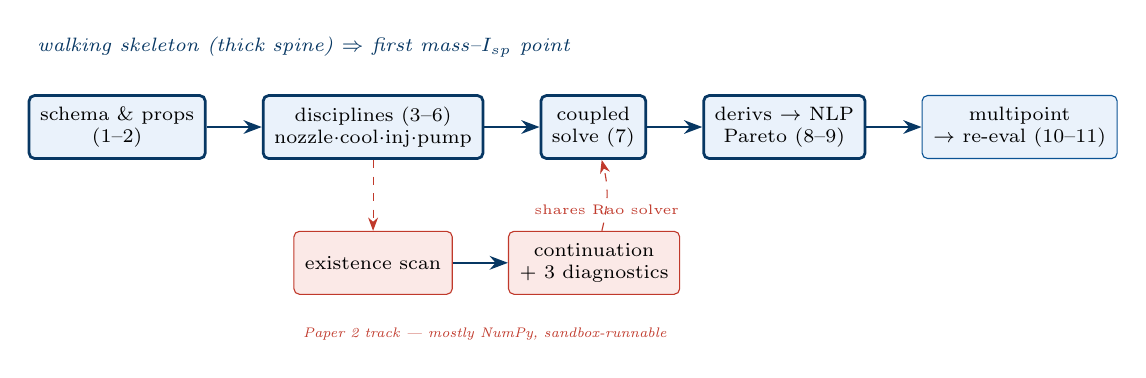
\begin{tikzpicture}[
  >={Stealth[length=2mm]},
  n/.style={draw=accent,fill=notebg,rounded corners=2pt,inner sep=4pt,
            font=\scriptsize,align=center,minimum height=8mm},
  sk/.style={draw=accentdark,fill=notebg,line width=1pt,rounded corners=2pt,
             inner sep=4pt,font=\scriptsize,align=center,minimum height=8mm},
  c/.style={draw=warnframe,fill=warnbg,rounded corners=2pt,inner sep=4pt,
            font=\scriptsize,align=center,minimum height=8mm},
  a/.style={accentdark,-{Stealth},thick},
  node distance=6mm and 7mm]
\node[sk] (n1) {schema \& props\\(1--2)};
\node[sk,right=of n1] (n2) {disciplines (3--6)\\nozzle$\cdot$cool$\cdot$inj$\cdot$pump};
\node[sk,right=of n2] (n3) {coupled\\solve (7)};
\node[sk,right=of n3] (n4) {derivs $\to$ NLP\\Pareto (8--9)};
\node[n,right=of n4] (n5) {multipoint\\$\to$ re-eval (10--11)};
\draw[a] (n1)--(n2); \draw[a] (n2)--(n3); \draw[a] (n3)--(n4); \draw[a] (n4)--(n5);
% cliff track (Paper 2), parallel
\node[c,below=9mm of n2] (ex) {existence scan};
\node[c,right=of ex] (co) {continuation\\+ 3 diagnostics};
\draw[a] (ex)--(co);
\draw[warnframe,dashed,-{Stealth}] (n2)--(ex);
\draw[warnframe,dashed,-{Stealth}] (co) to[bend right=14]
      node[below,font=\tiny]{shares Rao solver} (n3);
\node[font=\scriptsize\itshape,accentdark,anchor=west]
      at ([yshift=6mm]n1.north west) {walking skeleton (thick spine) $\Rightarrow$ first mass--$I_{sp}$ point};
\node[font=\tiny\itshape,warnframe,anchor=west]
      at ([yshift=-5mm]ex.south west) {Paper 2 track --- mostly NumPy, sandbox-runnable};
\end{tikzpicture}
\caption{Build-dependency graph. The thick spine is the walking skeleton to a
first mass--$I_{sp}$ point; the red track (existence boundary) builds on
\cmd{rao\_existence\_scan.py} and runs largely in parallel.}
\end{figure}

\noindent\textbf{MDO Pareto (Paper~1)} is the spine above: the mass--$I_{sp}$
frontier is generated by $\epsilon$-constraint sweeps in \cmd{nlp.py},
benchmarked against \cmd{design\_nozzle\_v2} (one-pass) and a block-coordinate
loop over the \emph{same} models (the fair baseline).
\textbf{Rao cliff (Paper~2)} builds on \cmd{rao\_existence\_scan.py} --- which
already encodes the smooth vs.\ fan/corner closures --- by adding
pseudo-arclength continuation and the three diagnostics of \S\ref{sec:cliff} as
\cmd{mdo/continuation.py}. It barely touches the MDO spine and is mostly
sandbox-runnable NumPy, so it de-risks independently.

\subsection{First increment (the walking skeleton)}
\begin{enumerate}[leftmargin=1.5em,itemsep=2pt]
\item \cmd{mdo/schema.py} $+$ \cmd{mdo/scaling.py}: the variable/bounds/mission
pytrees and a \cmd{jit}ed dummy \cmd{evaluate(x)} returning a scalar, so
\cmd{jax.jacfwd} runs clean (Phase-1 gate).
\item \cmd{mdo/properties.py}: tabulate \cmd{cea\_propellant} over $(P_c,O/F)$,
fit splines, validate gradients against held-out CEA points (Phase-2 gate).
\item \textbf{Skeleton \cmd{assembly.py}}: wire the analytic nozzle
(\cmd{primitives.py}) $+$ \cmd{throat\_wall\_temperature} $+$ algebraic injector
$+$ meanline pump into one $R$, solve with \cmd{least\_squares\_solve}, wrap in
\cmd{make\_differentiable\_solution}, and take \emph{one} end-to-end gradient.
That gradient existing is the real unlock; everything after deepens a block
behind a stable interface.
\end{enumerate}

\begin{warnbox}
\textbf{Reality checks.} JAX BVP solves are \emph{host-only} ($\sim$5--15\,min);
the implicit-contour path and full coupled solves run on your machine, not
in-session, while the analytic-contour skeleton is fast and testable anywhere.
Keep the NumPy oracle for every block so CI gates parity without the slow solves.
The honest long pole remains \textbf{J3b} (the differentiable kernel/BDE march),
but it gates \emph{only} wall-coordinate sensitivities on the implicit path --- the
skeleton and the Paper-1 Pareto do not wait on it.
\end{warnbox}

% =====================================================================
\section{Open risks and decision log}

\begin{enumerate}[leftmargin=1.5em,itemsep=3pt]
\item \textbf{Contour fidelity (decided).} TOP-B\'ezier for bulk Pareto;
implicit variational only for existence-boundary and exact-vs-TOP studies. J3b
(differentiable kernel/BDE march) gates \emph{only} wall-coordinate sensitivities
on the implicit path.
\item \textbf{Thermal fidelity ladder (decided).} 4a before 4b; do not gate first
coupled solves on quasi-2-D.
\item \textbf{$\cstar$ convention (decided).} $\cstar_\mathrm{delivered}=\eta_{\cstar}\cstar_\mathrm{ideal}$,
pinned in \cmd{properties.py}; no double counting in the injector closure.
\item \textbf{Coupling attribution (open).} No unique additive decomposition;
define an ablation protocol (freeze one feedback edge, re-optimize, measure
$\Delta$) and report order-dependence.
\item \textbf{Multipoint validity (open).} Evaluate separation, property, and
efficiency surfaces at \emph{every} operating point; deep throttle stresses the
separation screen and the off-BEP pump surface simultaneously.
\item \textbf{Coupled-state conditioning (open).} Feedback cycles make the
monolithic Newton solve stiff; budget homotopy/continuation for the state solve
itself, independent of the cliff study.
\item \textbf{SP-8089 opacity (noted).} Image scan; OCR required before any
correlation extraction.
\end{enumerate}

% =====================================================================
\begin{thebibliography}{99}
\small
\bibitem{rao1958} G.\,V.\,R.\ Rao, ``Exhaust Nozzle Contour for Optimum Thrust,''
\emph{Jet Propulsion} 28(6), 377--382, 1958. \cmd{propulsion\_texts/rao1958.pdf}.
\bibitem{rao1999} G.\,V.\,R.\ Rao, K.\ Beck, J.\ Booth, ``Nozzle Optimization for
Space-Based Vehicles,'' 1999. \cmd{propulsion\_texts/rao1999.pdf}.
\bibitem{raorecent} G.\,V.\,R.\ Rao, ``Recent Developments in Rocket Nozzle
Configurations,'' \emph{ARS J.}, 1961. \cmd{propulsion\_texts/RaoRecentDevinRockNozConfig.pdf}.
\bibitem{sp125} D.\,K.\ Huzel, D.\,H.\ Huang, \emph{Design of Liquid Propellant
Rocket Engines}, NASA SP-125. \cmd{propulsion\_texts/19710019929.pdf}.
\bibitem{sp8120} \emph{Liquid Rocket Engine Nozzles}, NASA SP-8120.
\cmd{propulsion\_texts/19770009165.pdf}.
\bibitem{sp8087} \emph{Liquid Rocket Engine Fluid-Cooled Combustion Chambers},
NASA SP-8087. \cmd{propulsion\_texts/19730022965.pdf}.
\bibitem{sp8089} \emph{Liquid Rocket Engine Injectors}, NASA SP-8089.
\cmd{propulsion\_texts/pintle\_injector/19760023196.pdf} (image scan).
\bibitem{sp8109} \emph{Liquid Rocket Engine Centrifugal Flow Turbopumps}, NASA
SP-8109. \cmd{propulsion\_texts/fuel\_pump\_design/19740020848.pdf}.
\bibitem{sp8052} \emph{Liquid Rocket Engine Turbopump Inducers}, NASA SP-8052.
\cmd{propulsion\_texts/fuel\_pump\_design/19710025474.pdf}.
\bibitem{sp194} \emph{Liquid Propellant Rocket Combustion Instability}, NASA
SP-194. \cmd{propulsion\_texts/19720026079.pdf}.
\bibitem{bartz1957} D.\,R.\ Bartz, ``A Simple Equation for Rapid Estimation of
Rocket Nozzle Convective Heat Transfer Coefficients,'' \emph{Jet Propulsion},
1957. \cmd{propulsion\_texts/technical-notes-1957.pdf}.
\bibitem{anderson} J.\,D.\ Anderson, \emph{Modern Compressible Flow}, McGraw-Hill.
\cmd{propulsion\_texts/5f36b7c4\dots.pdf}.
\bibitem{white} F.\,M.\ White, \emph{Fluid Mechanics}, 7th ed., McGraw-Hill.
\bibitem{pizzarelli2011} M.\ Pizzarelli, S.\ Carapellese, F.\ Nasuti, ``A
Quasi-2-D Model for the Prediction of the Wall Temperature of Rocket Engine
Cooling Channels,'' \emph{Numerical Heat Transfer A}, 2011.
\cmd{propulsion\_texts/pizzarelli2011.pdf}.
\bibitem{carlile1992} J.\ Carlile, R.\ Quentmeyer, ``An Experimental
Investigation of High-Aspect-Ratio Cooling Passages,'' AIAA, 1992.
\cmd{propulsion\_texts/carlile1992.pdf}.
\bibitem{son2017} M.\ Son et al., ``Design Procedure of a Movable Pintle
Injector for Liquid Rocket Engines,'' \emph{J.\ Propulsion and Power}, 2017.
\cmd{propulsion\_texts/pintle\_injector/son2017.pdf}.
\bibitem{son2015} M.\ Son et al., ``Effects of Momentum Ratio and Weber Number on
Spray Half Angles of a Pintle Injector,'' \emph{J.\ Thermal Science}, 2015.
\cmd{propulsion\_texts/pintle\_injector/s11630-015-0753-7.pdf}.
\bibitem{lee2021} J.\ Lee et al., ``Design and mass analysis of an electric-pump
feed system,'' \emph{Int.\ J.\ Aeronautical and Space Sciences}, 2021.
\cmd{propulsion\_texts/fuel\_pump\_design/s42405-020-00325-z.pdf}.
\bibitem{narloy1974} \emph{Low-Cycle Fatigue of NARloy-Z}, NASA CR-134627.
\cmd{propulsion\_texts/materials\_science/19740017910.pdf}.
\bibitem{porowski1985} J.\,S.\ Porowski et al., ``Simplified Design Methods for
Low-Cycle Fatigue of Thrust Chambers,'' 1985.
\cmd{propulsion\_texts/porowski1985.pdf}.
\bibitem{cea1311} S.\ Gordon, B.\,J.\ McBride, \emph{Computer Program for
Calculation of Complex Chemical Equilibrium Compositions and Applications},
NASA RP-1311, 1994.
\bibitem{martinsLambe2013} J.\,R.\,R.\,A.\ Martins, A.\,B.\ Lambe,
``Multidisciplinary Design Optimization: A Survey of Architectures,'' \emph{AIAA
J.} 51(9), 2013.
\bibitem{martinsHwang2013} J.\,R.\,R.\,A.\ Martins, J.\,T.\ Hwang, ``Review and
Unification of Methods for Computing Derivatives of Multidisciplinary
Computational Models,'' \emph{AIAA J.} 51(11), 2013.
\bibitem{hwangMartins2018} J.\,T.\ Hwang, J.\,R.\,R.\,A.\ Martins, ``A
Computational Architecture for Coupling Heterogeneous Numerical Models and
Computing Coupled Derivatives,'' \emph{ACM TOMS} 44(4), 2018.
\url{https://dl.acm.org/doi/10.1145/3182393}.
\bibitem{gray2019} J.\,S.\ Gray, J.\,T.\ Hwang, J.\,R.\,R.\,A.\ Martins, et al.,
``OpenMDAO: an open-source framework for multidisciplinary design, analysis, and
optimization,'' \emph{Struct.\ Multidiscip.\ Optim.} 59, 2019.
\url{https://link.springer.com/article/10.1007/s00158-019-02211-z}.
\bibitem{benchmark2020} ``Benchmarking of monolithic MDO formulations and
derivative computation techniques using OpenMDAO,'' \emph{Struct.\ Multidiscip.\
Optim.}, 2020.
\url{https://link.springer.com/article/10.1007/s00158-020-02521-7}.
\bibitem{martinsNing2021} J.\,R.\,R.\,A.\ Martins, A.\ Ning, \emph{Engineering
Design Optimization}, Cambridge Univ.\ Press, 2021.
\bibitem{blondel2022} M.\ Blondel et al., ``Efficient and Modular Implicit
Differentiation,'' NeurIPS 2022; arXiv:2105.15183.
\url{https://arxiv.org/pdf/2105.15183}.
\bibitem{optimistix2024} J.\ Rader, T.\ Lyons, P.\ Kidger, ``Optimistix: modular
optimisation in JAX and Equinox,'' arXiv:2402.09983, 2024.
\url{https://arxiv.org/pdf/2402.09983}.
\bibitem{keller1977} H.\,B.\ Keller, ``Numerical solution of bifurcation and
nonlinear eigenvalue problems,'' in \emph{Applications of Bifurcation Theory},
Academic Press, 1977.
\bibitem{wachter2006} A.\ W\"achter, L.\,T.\ Biegler, ``On the implementation of
an interior-point filter line-search algorithm for large-scale nonlinear
programming (IPOPT),'' \emph{Math.\ Program.} 106, 2006.
\bibitem{griewank2008} A.\ Griewank, A.\ Walther, \emph{Evaluating Derivatives},
2nd ed., SIAM, 2008.
\end{thebibliography}

\end{document}
